\section{Galaxies Colours and Host Contamination}
\subsection{Spectral Energy Distribution Modelling \& Fitting}
% SEDS and the relevance
The multi-wavelength emission of galaxies across the electromagnetic spectrum contains information about their physical properties and characteristics. These baryonic processes that govern a galaxy's evolution and describe its history are intrinsically tied to its spectral energy distribution (SED). A galaxy is a composite of its constituent stars, whose combined emission provides insights into a galaxy's star formation history \citep{tinsley_evolution_1980}. Nebular emission lines can be explained by gas being heated by young stars, and MIR and FIR emissions are a sign of heated dust in the interstellar medium (ISM; \citealt{da_cunha_simple_2008}). In addition, atomic emission or absorption lines can be used to determine galaxies' redshift and estimate their distances from Earth. While the SEDs contain much information required to study these galaxies, drastically different galaxies may have broadly similar SEDs. \\\\ Galaxies are complicated systems, and the complex interplay between the physical processes within the galaxy affects the overall shape of the galaxies observed SED. To accurately describe these galaxies, SED modelling and fitting techniques have been developed that allow stellar, dust, and gas components to be simultaneously modelled from multi-wavelength data to allow the true nature of these galaxies to be inferred \citep{walcher_fitting_2011, conroy_modeling_2013}. Stellar population modelling consists of combining multiple stellar templates \citep{bruzual_stellar_2003, eldridge_spectral_2009} that best reflect a galaxy's age and metallicity, using the most appropriate initial mass function (IMF) to describe the distribution of masses from which the stars are formed \citep{salpeter_luminosity_1955, chabrier_galactic_2003} and the assumption of a parameterised star-formation history (SFH; \citealt{carnall_how_2019}) to describe prior star-formation. In addition to models that account for the stellar emissions, light absorption due to dust attenuation must also be accounted for; this is usually done with dust attenuation models such as those from \cite{charlot_simple_2000} and \cite{calzetti_dust_2000}, which are widely used within the literature. Similarly, dust emission must be accounted for using dust and particle emission models \citep{draine_infrared_2007, dale_two-parameter_2014}. To account for the contribution of AGN to their host galaxy, models of AGN emission are frequently employed \citep{fritz_revisiting_2006, stalevski_dust_2016}. Together, these components allow for a relatively effective modelling of a galaxy spectrum. However, numerous issues within the literature still prevent a full understanding of the physical processes underlying these galaxy SEDs.\\\\ One of the biggest issues within the literature is the debate surrounding the best way to model complex star formation histories. While the process of star formation is complex, SED modelling uses parameterised SFH models with simple, functional forms such as exponential decay to model SFHs. \cite{leja_how_2019} argue that `non-parametric models may be able to produce more accurate and less biased results than parametric models'. In contrast, \cite{robotham_prospect_2020} argues that `well-chosen parametric models can produce comparable results to non-parametric SFH models'. Another important consideration is the potential variability of the IMF. \cite{kroupa_variation_2001} suggests `a universal IMF is plausible', rejecting the idea of redshift or environmental dependence for the IMF. In contrast, \cite{chabrier_galactic_2003} postulates a `weak dependence on the environment but is otherwise well constrained'. Alternatively, \cite{dokkum_evidence_2008} suggests that `an evolving IMF is plausible'. While it is not universally understood about the true nature of the IMF, \cite{hopkins_dawes_2018} presents a framework for considering the potential variations in the IMF to study the IMF further and potentially draw conclusions about its variability. Due to the variety of parameters that may arise when modelling the SED of galaxies, many software packages have been developed such as MAGPHYS \citep{da_cunha_simple_2008}, CIGALE \citep{boquien_cigale_2019}, BAGPIPES \citep{carnall_inferring_2018}, and PROSPECTOR \citep{leja_deriving_2017, johnson_stellar_2021}, all of which are widely used within the literature and allow for modelling of diverse spectral energies. SED fitting is a valuable tool in SED modelling and is used when the full SED isn't available; in cases like these, available broadband photometric data can be used and fit against SED templates and models that have been created to infer properties about the galaxy. Using this method, information can be extracted about the colour of galaxies and their physical properties can be derived \citep{walcher_fitting_2011}. This is exceptionally useful in studies of AGN as advances in SED modelling have allowed SEDs to be decomposed by separating active galaxies into their galaxy and AGN components \citep{yang_fitting_2022}.  
% Connecting sentence to colours and colour space
\subsection{Galaxy Colour-space and Colour-Colour Diagrams}
A galaxy's colour is largely determined by the types of stars it contains, the dust that may redden it, and other factors such as cosmological redshift. These factors influence the overall shape of a galaxy's SED, in which specific wavelength emissions may dominate. This is evident in QGs characterised by dominant IR emission, while SFGs generally are characterised by a dominant emission in the UV-Optical spectrum \citep{strateva_color_2001}. Figure \ref{fig:bimodalSEDs}
shows the characteristic red and blue colours of QGs and SFGs. 
\begin{figure}[h!]
    \centering
    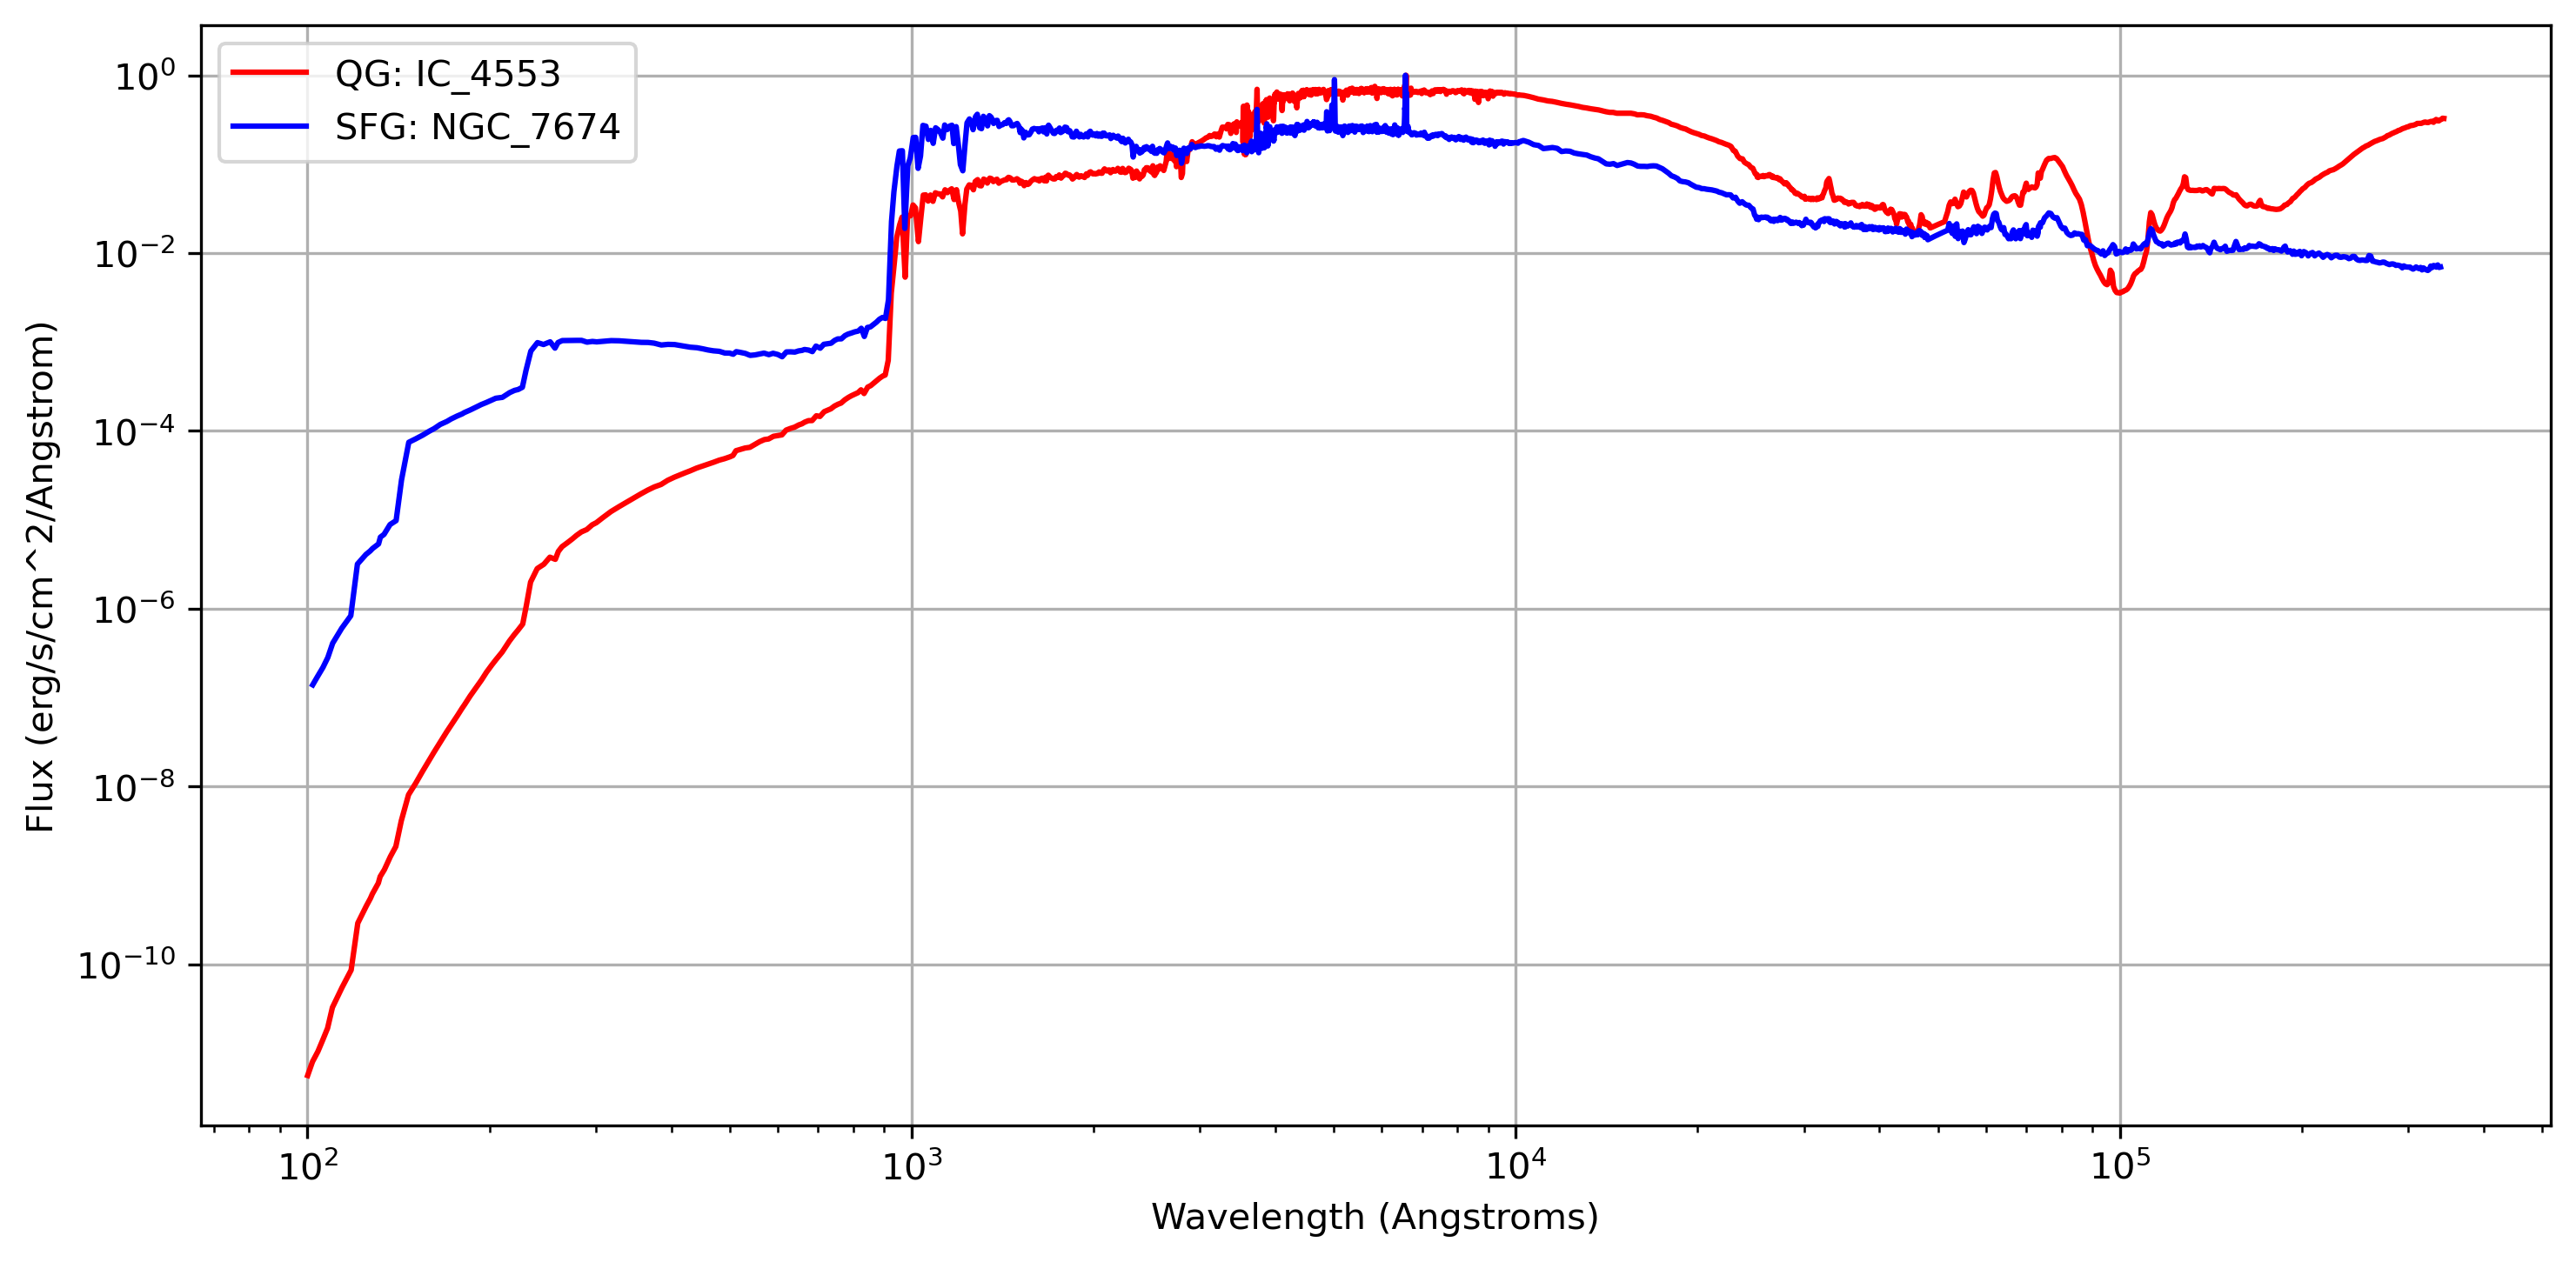
\includegraphics[width=1\textwidth]{Images/bimodalSEDs.png}
    \caption{Spectral Energy Distributions for the peculiar galaxy IC4553 and for the spiral galaxy NGC7674 taken from the GALSEDATLAS template library \citep{brown_atlas_2014}.}
    \label{fig:bimodalSEDs}
\end{figure} 
\\ In general, the colour of a galaxy is quantified in terms of its colour index, C, where the colour index is the difference in magnitudes between two distinct photometric bands. The colour index, therefore, measures the relative intensity between the two different magnitudes \citep{ballesteros_new_2012} and can be calculated using the equation below:
\begin{align}
    C = M_1 - M_2 = -2.5log_{10}\left(\frac{f_1}{f_2}\right)
\end{align}
Where $M_1$ and $M_2$ represent the absolute magnitudes, while $F_1$ and $F_2$ are fluxes associated with each magnitude in each band. Calculating this colour index is essential and forms the basis for analysing stellar and galactic properties using colour-colour diagrams. Colour-colour diagrams rely on constructing a plot of two colour indices. They can be constructed with either observed colours, whereby the colour index is derived from directly observed flux, or using rest-frame colours, for which the effect of cosmological redshift is accounted. Many different types of colour-colour diagrams are used for various purposes in the literature. Colour-colour diagrams have been used to select AGN \citep{lacy_obscured_2004, messias_dependency_2014, donley_spitzer_2007}, determine redshift \citep{giavalisco_lyman-break_2002}, and to separate star-forming forming galaxies from quiescent galaxies \citep{whitaker_newfirm_2011}. The UVJ colour-colour selection diagram is one such tool that utilises rest-framed UV, Optical and Near-Infrared (NIR) photometric fluxes \citep{whitaker_newfirm_2011} to correct for the effects of redshift and exploit their intrinsic bimodal colour behaviour. Techniques such as the UVJ diagram utilise boundaries to separate galaxies based on where they sit on the diagram (See Figure \ref{fig:colour-colour-diagram}).
\begin{figure}[h!]
    \centering
    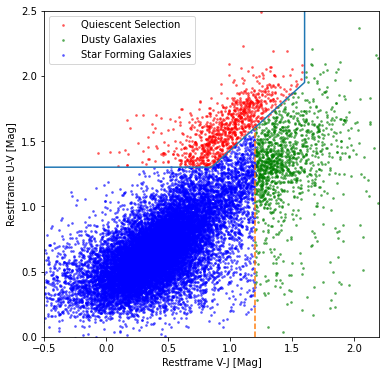
\includegraphics[width=0.5\textwidth]{Images/ZFOURGE_UVJ.png}
    \caption{A UVJ Diagram separating quiescent, star-forming and dusty galaxies using photometric data from the ZFOURGE Survey. The bi-modal colour behaviour of these galaxies is utilised to separate the sources, with sources on the right being attributed to QGs or dust-reddened sources.}
    \label{fig:colour-colour-diagram}
\end{figure} 
AGN colour-colour selection, like the Lacy Wedge \citep{lacy_optical_2007}, identifies potential AGNs by isolating them within specific regions of a colour-colour diagram based on their distinct MIR emission. Redshift determination colour-colour selection techniques similarly use a selection area. The most widely used redshift determination technique in the literature is the Lyman-break technique, in which the Lyman-break of galaxies is used to determine if a galaxy is at a particular redshift based on the observed wavelength at which photons are completely absorbed by hydrogen gas \citep{giavalisco_lyman-break_2002}. The strength of these colour selection techniques is that they can utilize limited photometric data to infer galaxy properties, requiring only three bandpass filters to construct the colour-colour diagram. The strength of these techniques is also one of their limitations, as relying solely on limited data points may cause broadly similar sources to be incorrectly identified due to slight changes in their colours, thus contaminating the colour space. \cite{patel_uvj_2012} suggests that introducing even the slightest amount of star formation on top of a QG population may move the galaxies from the quiescent to star-forming regions in the UVJ diagram. In contrast, \cite{newman_photometric_2022} discusses the reduced efficacy of the Lyman break technique in galaxies with high metallicity stars. Likewise, AGN colour-colour selection techniques similarly suffer from many contamination issues. Most notable in the literature is the effect of PAH emission from SFGs mimicking the colours of AGN; this is discussed in more detail in \cite{hickox_obscured_2018}. Colour space contamination is a common theme amongst colour-colour selection techniques and is well recognised throughout the literature as a major limitation of these techniques. 
\subsection{AGN Contamination}
Due to the highly luminous contribution of an AGN to their host galaxy, determining the physical properties of a host galaxy, such as star formation rate, history and stellar masses, can be very difficult \citep{kauffmann_host_2003}. Throughout the literature, there are varying claims about the exact level of contamination to host galaxies, with \cite{salim_uv_2007} suggesting that UV emission can cause a gross overestimation in SFR. In contrast, \cite{cowley_zfourge_2016} highlights that contamination from AGN can introduce systematic errors when calculating SFRs derived from IR+UV emissions due to excess IR emission. \cite{cowley_zfourge_2016} adds that `AGN contamination in the UV range is unlikely to cause substantial changes to the calculated SFR'. \cite{ciesla_constraining_2015} argued that `properties derived from galaxies containing Type 1 AGN would be significantly overestimated', with stellar masses being overestimated by up to $150\%$ and SFRs being overestimated by up to 300\%. As both stellar mass and star formation are derived properties from a galaxy SED, we can see how an increasing AGN presence in a galaxy can cause a drastic change in the SED (See Figure \ref{fig:sed_agn_contaminiation}) affecting the derived properties.
\begin{figure}[h!]
    \centering
    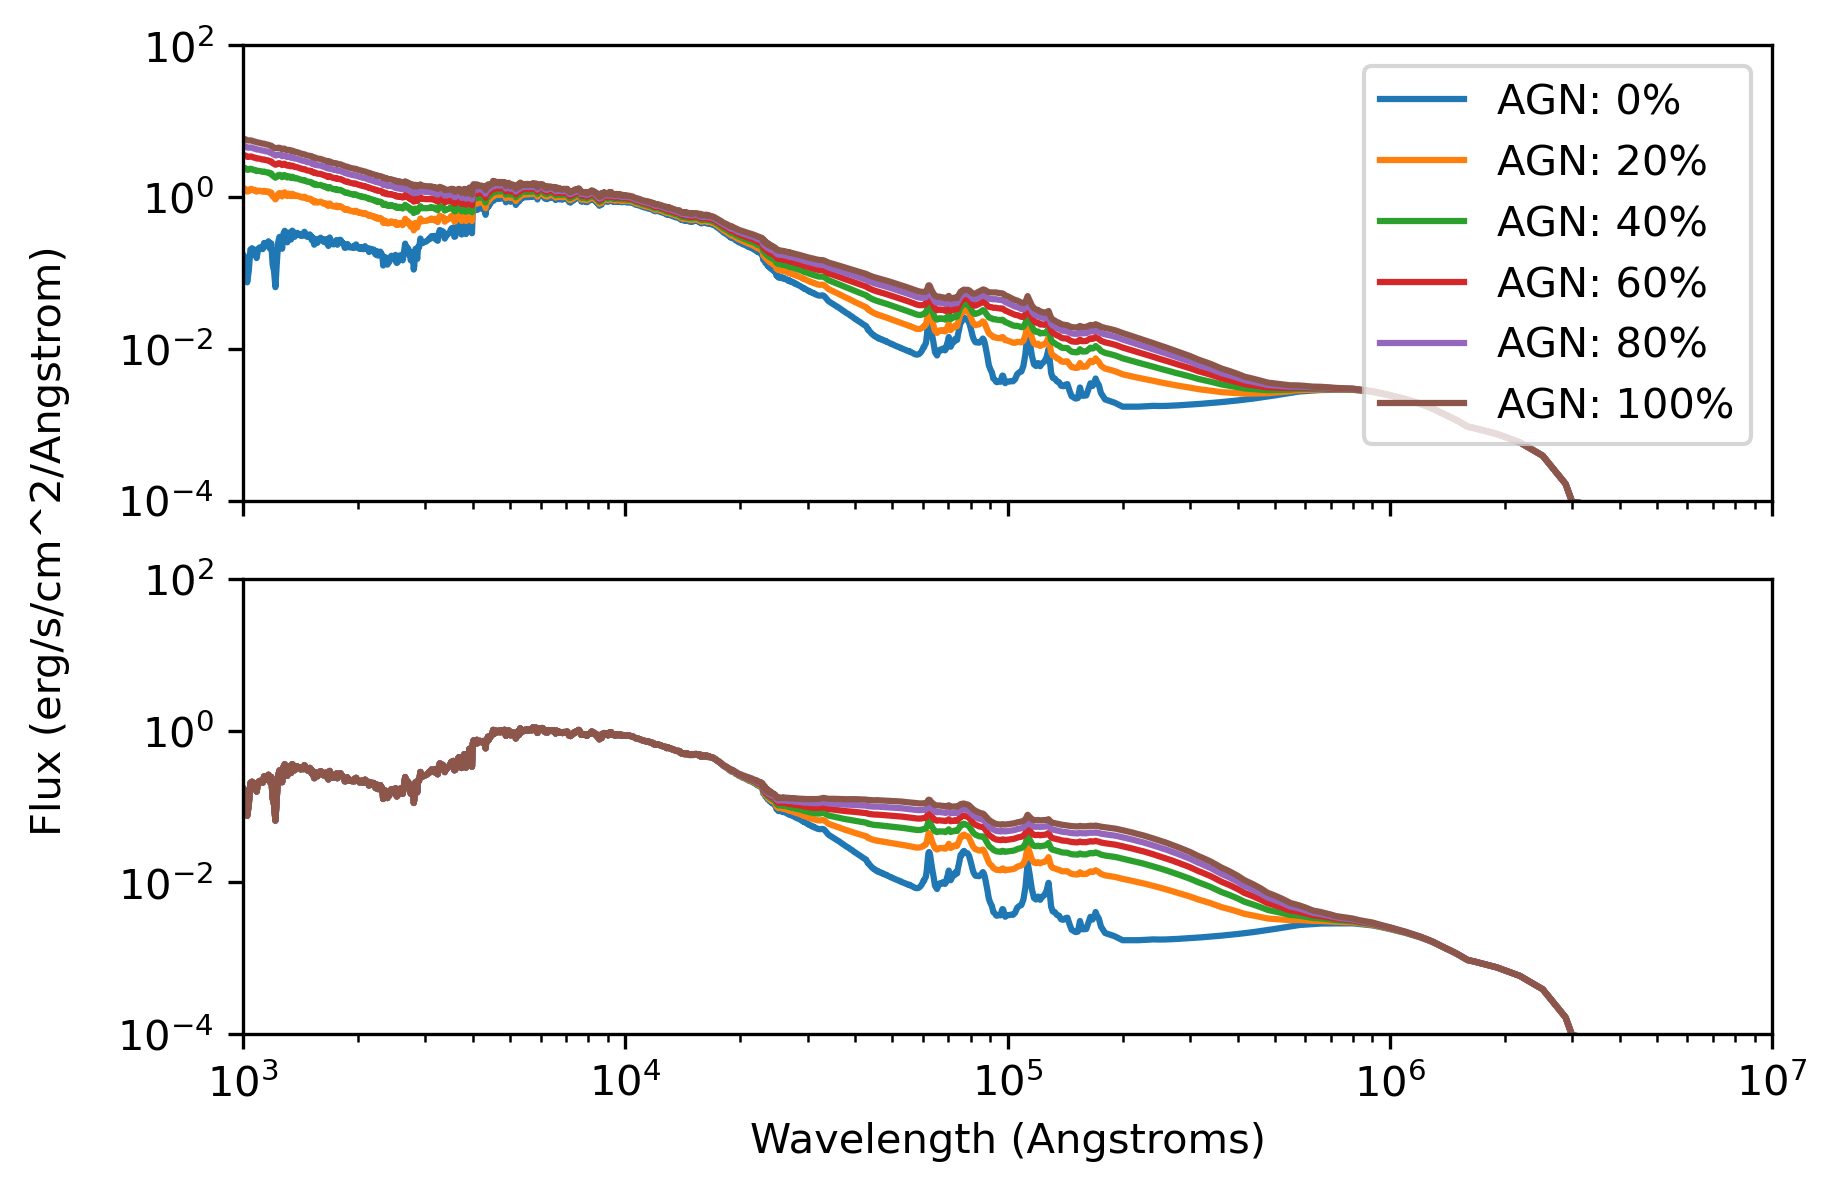
\includegraphics[width=0.8\textwidth]{Images/sed_agn_contaminiation_updated.png}
    \caption{Type 1 (Top) and Type 2 (Bottom) Composite SEDs constructed using SWIRE templates \citep{polletta_spectral_2007} and the Skirtor AGN Models \citep{stalevski_dust_2016}. Bluer colours characterize type 1 AGN due to the lack of an obscuring torus; thus, a drastic increase in UV-optical light is observed in the SED}
    \label{fig:sed_agn_contaminiation}
\end{figure}\\\\There is a drastic change in the overall SEDs when Type 1 and Type 2 AGN are present within a galaxy. In particular, there is a noticeable increase in UV-optical colours due to the line of sign towards the accretion disk for galaxies with a Type 1 AGN. Meanwhile, the obscuring torus-dominated emission causes galaxies to display an IR excess. Naturally, this will affect the colour space of galaxies, contaminating the colour-colour diagram and disrupting the bi-modality of galaxies. \cite{brown_spectral_2019} briefly explores this effect by modelling the spectral energies of galaxies without an AGN component and then gradually adding the component in. The author finds that in doing so, the composite galaxies plotted on colour-colour diagrams eventually trace paths to a quasar locus. While there is a notable change in galaxy colours due to a sufficiently luminous AGN component, there is no consensus for dealing with or interpreting AGN in colour-colour diagnostics. \cite{diaz-garcia_stellar_2019} includes AGN in the UVJ analysis of galaxies, finding that AGN host galaxies are generally present in the quiescent galaxies, likening this result to be an indicator of star-formation quenching. Conversely, \cite{fang_demographics_2018} also explores the demographics of galaxies using colour-colour diagnostics, while \cite{kawinwanichakij_distribution_2014} analyses the distribution of satellites around massive galaxies, with neither considering the effect of AGN on the sample. As AGN is present in most massive galaxies, explicit consideration in colour diagnostics is necessary. Failure to do so may result in erroneous conclusions regarding these galaxies' stellar populations, star formation histories, and overall evolutionary pathways.
